\chapter{Poisson's Equation}\label{ch:poisson-eq}
\begin{chout}
	We reach the main chapter of the report, and prove\sidenotemark\ a deep,
	analytic result for the to-be-defined Laplacian operator.
\end{chout}
\sidenotetext[][5\baselineskip]{\footnotesize\cite{donaldson}}

\section{Laplace operator}
To give context to the developments of the chapter, it makes sense to state the
result which we ultimately aim to prove. In order to state this result however,
it is necessary to define the Laplacian operator.

\begin{definition}[Laplacian]
	For a Riemann surface $ X $, we define the \defined{Laplacian} to be the
	differential operator
	\begin{align*}
		\Delta: \Omega^0(X) \to \Omega^2(X):f \mapsto 2i
		\overline{\partial}\partial f,
	\end{align*}
	and say that the function $ f $ is \defined{harmonic} if it satisfies,
	\begin{align*}
		\Delta f = 0.
	\end{align*}
\end{definition}

\begin{remark}
	This definition is chosen specifically such that it agrees, in local
	coordinates, with the familiar representation of the Laplace operator as
	\begin{align*}
		\Delta f & = \frac{2i}{4} \left( \frac{\partial }{\partial x}+ i
		\frac{\partial }{\partial y} \right)\left( \frac{\partial }{\partial x}- i
		\frac{\partial }{\partial y} \right) f \d{z}\d{\overline{z}}            \\
		         & = - \left( \frac{\partial^2 }{\partial x^2}+\frac{\partial^2
		}{\partial y^2} \right)f \d{x}\d{y}.
	\end{align*}
\end{remark}

\begin{theorem}\label{thm:fredholm}
	Let $ X $ be a compact Riemann surface and let $ \rho \in \Omega^2(X) $. There
	exists a function $ f \in \Omega^0(X) $ such that $ \Delta f = \rho $ if and
	only if
	\begin{align*}
		\int_{X}{\rho} = 0
	\end{align*}
	and this solution is unique up to an additive constant.
\end{theorem}

The above theorem is referred to as the `Main Theorem' in
Donaldson\sidenote{\footnotesize\cite[p. 113]{donaldson}}. Intuitively, we can
think of this statement as giving the necessary and sufficient conditions to
invert the Laplacian, i.e., solve Poisson's equation, on a compact Riemann
surface.

Initial progress on the proof of Theorem~\ref{thm:fredholm} is easy to come by,
in particular in the `if' direction.

\begin{lemma}
	If there exists a function $ f $ such that $ \Delta f = \rho $,
	\begin{align*}
		\int_{X}{\rho} = 0.
	\end{align*}
	\begin{proof}
		This is a corollary to Stokes' theorem.
		\begin{align*}
			\int_{X}{\rho}  = \int_{X}{\Delta f}
			= 2i \int_{X}{\overline{\partial}\partial f}
			= 2i \int_{X}{\d{\left( \partial f \right)}}
			= 2i \int_{\varnothing}{\partial f} = 0
		\end{align*}
	\end{proof}
\end{lemma}

\begin{lemma}
	If there exists a function $ f $ such that $ \Delta f = \rho $, this function
	is unique up to addition by a constant.
	\begin{proof}
		A simple argument based on maximum modulus principle.
	\end{proof}
\end{lemma}

So, the interesting content in Theorem~\ref{thm:fredholm} can be summarised as
the following.

\begin{theorem}\label{thm:main-thm}
	If $ \rho \in \Omega^2(X) $ is such that
	\begin{align*}
		\int_{X}{\rho} = 0,
	\end{align*}
	there exists a function $ f $ such that $ \Delta f = \rho $.
\end{theorem}

This is the result we aim to prove in the proceeding sections.

\section{Dirichlet norm}
\begin{definition}[$ L^2 $ inner product]
	Let $ \alpha, \beta \in \Omega ^{1,0}(X) $. Then, we define the \defined{$ L^2
		$ inner product} to be,
	\begin{align*}
		\left\langle \alpha, \beta \right\rangle _{L^2} = \int_{X}{i \alpha \wedge
			\overline{\beta}}.
	\end{align*}
\end{definition}

To show that this is definition is more familiar than is superficially obvious,
let us consider a local coordinate $ z=x+iy $ in which $ \alpha $ and $ \beta $
are expressible as $ f(z) \d{z} $ and $ g(z) \d{z} $ respectively. Then,
\begin{align*}
	\left\langle \alpha, \beta \right\rangle _{L^2} & = \int_{X}{i \alpha\wedge
	\overline{\beta}}                                                           \\
	                                                & = i\int_{X}{\left( f(z)
		\d{z} \right)\wedge
		\overline{\left( g(z)\d{z}
	\right)}}                                                                   \\
	                                                & = i\int_{X}{f(z)
	\overline{g(z)}\d{z}\d{\overline{z}}}                                       \\
	                                                & = 2\int_{X}{f
		\overline{g}\d{x}\d{y}},
\end{align*}

and we can define the associated norm,
\begin{align*}
	\|\alpha\|_{L^2}^{2} = \left\langle \alpha,\alpha \right\rangle _{L^2} =
	\int_{X}{i \alpha \wedge \overline{\alpha}} = 2\int_{X}{|f|^{2}\d{x}\d{y}},
\end{align*}
which we refer to as the \defined{$ L^2 $ norm}.

\begin{lemma}
	$ \|\cdot \|_{L^2} $ defines a norm on the compactly supported $ (1,0)
	$-forms.
	\begin{proof}
		There is little to note apart from the fact that compactness ensures the
		finiteness of the defining integral.
	\end{proof}
\end{lemma}

\begin{remark}
	The main observation here is that the $ L^2 $ inner product (and also $ L^{2}
	$ norm) is coordinate independent.
\end{remark}

We can easily extend our definition for the $ L^2 $ inner product (and
consequently norm) to the $ C ^{\infty} $ $ 1 $-forms, by associating these with
their $ (1,0) $ component. In particular, let $ A,B \in \Omega^1(X) $, then,
\begin{gather*}
	\left\langle A,B \right\rangle _{L^2} = 2 \left\langle A ^{1,0}, B ^{1,0}
	\right\rangle _{L^2} = 2i \int_{X}{A ^{1,0}\wedge B ^{0,1}},\\
	\left\|A\right\|_{L^2}^{2} = 2\left\|A^{1,0}\right\|_{L^2}^{2}.
\end{gather*}

\begin{definition}[Dirichlet inner product]
	Let $ f,g:X \to \mathbb{R} $ be $ C ^{\infty} $, at least one compactly
	supported. The \defined{Dirichlet inner product} is defined as
	\begin{align*}
		\left\langle f,g \right\rangle _{\mathcal{D}} = \left\langle \d{f}, \d{g}
		\right\rangle _{L^2},
	\end{align*}
	and similarly, the \defined{Dirichlet norm} is defined as,
	\begin{align*}
		\|f\|_{\mathcal{D}} = \| \d{f}\|_{L^2}.
	\end{align*}
\end{definition}

\begin{remark}
	We note that the Dirichlet `norm' is in fact a `semi-norm', since it is
	positive semi-definite rather than definite. We can see this by noting that
	the constant functions all have zero derivative. As a result of this, it is
	common to consider the space of functions $ C ^{\infty}(X,
		\mathbb{R})/\mathbb{R} $, i.e., the quotient of the space of $ C ^{\infty} $
	functions on $ X $ by the constant functions.
\end{remark}

\begin{lemma}
	If at least one of $ f,g $ have compact support,
	\begin{align*}
		\left\langle f,g \right\rangle _{\mathcal{D}} = \int_{X}{f \Delta g} =
		\int_{X}{g \Delta f}.
	\end{align*}
	\begin{proof}
		Following from the definitions outlined above, and recalling that $ f $ and $
			g$ are real valued gives,
		\begin{align*}
			\left\langle f,g \right\rangle _{\mathcal{D}} & = \left\langle \d{f}, \d{g}
			\right\rangle _{L^2}                                                        \\
			                                              & = 2i \int_{X}{\partial f
				\wedge \overline{\partial
			g}}                                                                         \\
			                                              & = 2i \int_{X}{\partial f
				\wedge \overline{\partial }g}.
		\end{align*}
		Then, integrating by parts gives,
		\begin{align*}
			2i\int_{X}{\partial f \wedge \overline{\partial}g} & = 2i \int_{X}{\partial
				\left( f \overline{\partial}g \right) - f \partial
				\overline{\partial}g}.
		\end{align*}
		Finally, applying Stokes' theorem to the first term in this expression,
		\begin{align*}
			2i \int_{X}{\partial \left( f \overline{\partial}g \right)} - 2i
			\int_{X}{f\partial \overline{\partial}g} & = -2i \int_{X}{f \partial
			\overline{\partial}g}                                                \\
			                                         & = 2i \int_{X}{f
			\overline{\partial}\partial g}                                       \\
			                                         & = \int_{X}{f \Delta g}.
		\end{align*}
	\end{proof}
\end{lemma}

\section{Changing viewpoint}
It is at this point natural to ask how the constructions introduced in the
previous section help us in proving Theorem~\ref{thm:main-thm}. We now dedicate
some time to explore this question in detail, ultimately repackaging the
information contained in Theorem~\ref{thm:main-thm} to something more
appropriate.

To begin, let us denote by $ H $, the space $ C
		^{\infty}(X;\mathbb{R})/\mathbb{R} $, which is an inner product space with
respect to the Dirichlet inner product.

\begin{remark}
	In particular, the inner product $ \left\langle \cdot , \cdot  \right\rangle
		_{\mathcal{D}} $ is positive definite in this case, since the constant functions
	are identified with the class which may be represented by the zero function, $
		\left[ 0 \right] $. Moving forward, we will not make explicit distinction
	between a function $ \psi \in C ^{\infty}(X;\mathbb{R}) $ and the equivalence
	class of functions represented by $ \left[ \psi \right] \in C
			^{\infty}(X;\mathbb{R})/\mathbb{R} $, since this distinction does little
	more than contribute notative complexity to the discussion.
\end{remark}

It is clear that for $ f \in H $, $ \rho \in
	\Omega^2(X) $, the statement $ \Delta f = \rho $ is equivalent to
\begin{align*}
	\int_{X}{g \left( \rho - \Delta f \right)}=0
\end{align*}
for every function $ g \in C ^{\infty}(X ;\mathbb{R}) $. Furthermore,
\begin{align*}
	\int_{X}{g \left( \rho - \Delta f \right)} & = \int_{X}{g \rho} - \int_{X}{g
	\Delta f}                                                                      \\
	                                           & = \int_{X}{g \rho} - \left\langle
	g,f\right\rangle _{\mathcal{D}}.
\end{align*}

Consider now the functional defined by
\begin{align*}
	\tilde{\rho} & : C ^{\infty}(X; \mathbb{R}) \to \mathbb{R} \\
	             & : g \mapsto \int_{X}{\rho g},
\end{align*}
and suppose that $ \int_{X}{\rho} = 0 $ as in the hypothesis of
Theorem~\ref{thm:main-thm}. We claim that this functional descends to a linear
functional on $ H $, which is justifiable by the following. Let $ g \sim g' $ in
$ C ^{\infty}(X;\mathbb{R})/\mathbb{R} $, that is let $ g = g' + c $ for some $
	c \in \mathbb{R}$. Then,
\begin{align*}
	\tilde{\rho}(g) = \int_{X}{\rho g}
	= \int_{X}{\rho \left( g' + c \right)}
	= \int_{X}{\rho g'} + \int_{X}{\rho c}
	= \int_{X}{\rho g'}
	= \tilde{\rho} (g').
\end{align*}

Hence, we define the descended functional,
\begin{align*}
	\hat{\rho} & : H \to \mathbb{R}                          \\
	           & : \left[ g \right] \mapsto \int_{X}{\rho g}
\end{align*}
which allows us to repackage the information contained in
Theorem~\ref{thm:main-thm}.

\addtocounter{definition}{-5}
\begin{theorem}
	If $ \rho \in \Omega^2(X) $ is such that
	\begin{align*}
		\int_{X}{\rho} = 0,
	\end{align*}
	there exists a function $ f $ such that
	\begin{align*}
		\hat{\rho}(g) = \left\langle g,f \right\rangle _{\mathcal{D}}
	\end{align*}
	for all $ g \in H $.
\end{theorem}
\addtocounter{definition}{4}

\section{Riesz representation theorem}\label{sec:riesz}
The previous section seems to have done little for progress aside from change
the framework in which our problem is stated. This is, however, an important
shift, and brings us to a well known result from functional analysis, which will
prove integral.

\begin{theorem}[Riesz representation theorem]\label{thm:riesz}
	Let $ \sigma: \mathcal{H}\to \mathbb{R} $ be a bounded linear function on a
	real Hilbert space $ \mathcal{H} $. Then, there exists an element $ z \in
		\mathcal{H} $, such that
	\begin{align*}
		\sigma(x) = \left\langle z,x \right\rangle
	\end{align*}
	for all $ x \in \mathcal{H} $.
\end{theorem}

Let us now consider the obstacles between our current position and application
of this theorem.
\begin{enumerate}
	\item The functional $ \hat{\rho} $ may not be bounded.
	\item The space $ H $ is not a Hilbert space.
\end{enumerate}

We address these issues in turn.

\subsection{Boundedness of $ \hat{\rho} $}
In order to show the boundedness of $ \hat{\rho} $, we aim to apply a well known
result due to Poincar\'e.

\begin{proposition}[Poincar\'e inequality]\label{prop:poincare-ineq}
	Let $ D \subset \mathbb{R}^{2} $ be a circular disc of area $ A $. Then for $
		\psi $ defined on a superset of $ \overline{D} $, there exists a constant $ C
	$ such that
	\begin{align*}
		\| \psi - \psi_D \|_{L^2 ( D )} \leq C \| \nabla \psi \|_{L^2 ( D )},
	\end{align*}
	where $ \psi_D $ denotes the average of $ \psi $ over $ D $,
	\begin{align*}
		\psi_D = \frac{1}{A}\int_{D}{\psi ( y )}\d{y}.
	\end{align*}
\end{proposition}

\begin{marginfigure}
	\centering
	\includegraphics{convex/figure}
	\caption{Proposition~\ref{prop:poincare-ineq} actually holds for any bounded
		convex set $ C $, but we need only consider the case of the disc. Above is a
		convex set $ C $, and a non-convex set $ N $.}
\end{marginfigure}


\begin{remark}
	For reasons related to \defined{partitions of unity} and an isomorphism between
	the second de Rham group and $ \mathbb{R} $, it suffices to show that $
		\hat{\rho} $ is bounded when it is supported in a given chart of the Riemann
	surface\sidenotemark.
\end{remark}
\sidenotetext{\footnotesize\cite[p. 125]{donaldson}}

Let $ (U, \phi) $ be a chart, such that $ \supp \rho \subset U $, and by
homeomorphism identify its image $ \tilde{U} $ with a circular disc $ D $ of
area $ A $. We have a local coordinate system $ ( x,y ) $ on $ D $ afforded to
us by the coordinate map $ \phi $, and in this system, we can consider $ \rho $
as a function of integral $ 0 $, supported on $ D $, and $ \psi $ as a function
(initially on $ X $) defined on some superset of $ \overline{D} $.

These identifications allow us to express the functional in this local
coordinate as
\begin{align*}
	\hat{\rho}( \psi ) = \int_{D}{\rho \psi}\d{x}\d{y},
\end{align*}
which is equivalently expressed as
\begin{align*}
	\hat{\rho}( \psi ) = \int_{D}{\rho ( \psi - \psi_D )}\d{x}\d{y},
\end{align*}
since the integral of $ \rho $ is zero. This is exactly, the form (up to
scaling) of the $ L^2 $ norm introduced earlier, and as such, we can utilise the
Cauchy-Schwarz inequality to state that,
\begin{align*}
	\left| \int_{D}{\rho ( \psi-\psi_D )}\d{x}\d{y} \right| \leq \| \rho
	\|_{L^2(D)}\| \psi-\psi_D \|_{L^2(D)}.
\end{align*}
A final series of relations, the first justified by
Proposition~\ref{prop:poincare-ineq}, and the last by definition,
\begin{align*}
	| \hat{\rho}( \psi ) | \leq C \| \nabla \psi \|_{L^2 ( D )}
	\leq \| \nabla \psi \|_{L^2 ( X )} = C \| \psi \|_{\mathcal{D}}
\end{align*}
proves the boundedness of the functional in $ U $ and, by the above remark, on
$ X $.

\subsection{Completion}
We know that the functional $ \hat{\rho} $ is bounded, and hence it remains to
find a Hilbert space which is related to $ H $. We do this via the abstract
completion.

\begin{definition}[Completion]
	For an inner product space $ H $, with the inner product $ \left\langle \cdot
		,\cdot \right\rangle $ and the associated norm $ \|\cdot \| $, the
	\defined{completion} of $ H $ with respect to $ \| \cdot \| $, is a set of
	equivalence classes of Cauchy sequences $ \left( g_i \right) \in H $ where,
	\begin{align*}
		\left( g_i \right)\sim \left( g_i' \right) \iff \|g_i - g_i'\| \to 0.
	\end{align*}
\end{definition}

We denote by $ \mathcal{H} $ the completion of $ H $ with respect to the
Dirichlet norm $ \|\cdot\|_{\mathcal{D}} $. At this stage, application of the
Riesz representation theorem is obstructed solely by the fact that our
functional $ \hat{\rho} $ is defined on $ H $, rather than $ \mathcal{H} $. The
following result helps us solve this minor issue.

\begin{lemma}
	Let $ U,V $ be two normed spaces with respective norms $ \|\cdot \|_{U} $ and
	$ \|\cdot \|_{V} $, and consider the linear map $ \sigma:U \to V $. If $
		\sigma $ is bounded, then $ \sigma(u_i) $ is a Cauchy sequence in $ V $ for
	any Cauchy sequence $ (u_i) $ in $ U $.
	\begin{proof}
		We recall that the boundedness of the linear map $ \sigma $ is definitively
		equivalent to the existence of a constant $ C $ such that
		\begin{align*}
			\|\sigma(u)\|_{V} \leq C \|u\|_{U}
		\end{align*}
		for all $ u \in U $. Since $ (u_i) $ is Cauchy,
		\begin{align*}
			\|u_n - u_m\|_{U} \to 0
		\end{align*}
		as $ n,m \to \infty $, and hence
		\begin{align*}
			\|\sigma(u_n) - \sigma(u_m)\|_{V} & = \|\sigma(u_n-u_m)\|_{V}    \\
			                                  & \leq C \|u_n-u_m\|_{U} \to 0
		\end{align*}
		as $ n,m \to \infty $.
	\end{proof}
\end{lemma}

In our setting, this result determines that the sequence $ \hat{\rho}(g_i) $ is
Cauchy in $ \mathbb{R} $, and hence convergent. As a result, we can define the
extension of $
	\hat{\rho} $ by,
\begin{align*}
	\hat{\rho} & : \mathcal{H} \to \mathbb{R}                             \\
	           & : [(g_i)] \mapsto \lim _{i \to \infty}{\hat{\rho}(g_i)},
\end{align*}
which is a bounded linear map as needed. We choose to denote the extended
functional in the same way as the original functional, since these are so
closely related. Finally, we are in a position to apply Theorem~\ref{thm:riesz},
and can assert the existence of $ f \in \mathcal{H} $ such that
\begin{align*}
	\hat{\rho}(g) = \left\langle f,g \right\rangle _{\mathcal{D}}
\end{align*}
for all $ g \in \mathcal{H} $. A solution of this type is called a \defined{weak
	solution}, and for the proof of Theorem~\ref{thm:main-thm} we must show that
this weak solution is in fact a valid, smooth solution.

\section{Weyl's Lemma}
The following section concerns itself with the proof of a version of Weyl's
lemma, which will tie up the proof of Theorem~\ref{thm:main-thm}, in that it
will determine that any weak solution is smooth.

\begin{proposition}[Weyl's Lemma]\label{prop:weyl}
	Let $ D \subseteq \mathbb{C} $ be a bounded, open set, and let $ \rho \in
		\Omega^2(D) $. If $ \phi \in L^{2}(D) $, such that
	\begin{align*}
		\int_{D}{\chi \Delta \phi} = \int_{D}{\chi \rho}
	\end{align*}
	for all compactly supported, smooth functions $ \chi $, $ \phi $ is smooth,
	and satisfies $ \Delta \phi = \rho $.
\end{proposition}

\subsection{Relation to an $ L^{2} $ function}
To reiterate our current position, we have found a weak solution to the Posson
equation, $ f \in \mathcal{H} $ which is a Cauchy sequence $ ( f_{i} ) $ with
respect to $ \| \cdot  \|_{\mathcal{D}} $ such that, for any $ g $,
\begin{align*}
	\left\langle f_{i},g \right\rangle \to \hat{\rho}( g )
\end{align*}
as $ i \to \infty $. In order to apply Proposition~\ref{prop:weyl} we aim to
associate the Cauchy sequence with a locally $ L^{2} $ function. We first
consider this association in a single coordinate chart $ ( U, \phi ) $, and
identify $ \phi ( U ) $ with a bounded open set $ D \subseteq \mathbb{C} $.
Since the underlying collection of functions $ H $ of our completion $
	\mathcal{H} $ is $ C^{\infty}( X;\mathbb{R} )/\mathbb{R} $, we may freely add
constants to the functions $ f_{i} $ such that their integral vanishes over the
region $ D $. In particular, we can ensure that the average $ [ f_{i} ]_{D}=0 $.
Then,
\begin{align*}
	\left\| f_{n}-f_{m} \right\|_{L^{2}(D)} & = \left\| f_{n}-f_{m} -
	[ f_{n}-f_{m} ]_{D} \right\|_{L^{2}(D)}                                       \\
	                                        & \leq \left\| \nabla ( f_{n}-f_{m} )
	\right\|_{L^{2}(D)}                                                           \\
	                                        & \leq \left\| f_{n}-f_{m}
	\right\|_{\mathcal{D}} \to 0
\end{align*}
as $ n,m \to \infty $,which is enough to declare $ ( f_{i} ) $ as Cauchy in $
	L^{2} $. Furthermore, since $ L^{2}(D) $ is complete, $ ( f_{i} ) $ converges to
some function $ f \in L^{2}(D) $.

\begin{lemma}
	The sequence of functions $ ( f_{i} ) $ converges locally in $ L^{2} $ on $ X $.
	\begin{proof}
		We now aim to extend our above argument to account for all coordinate
		charts.

		Let $ A $ be the collection of points $ x \in X $ such that there exists a
		coordinate chart $ U_{x} $ in which $ \phi_{i}\to \phi$ with respect to $
			\|\cdot \|_{L^{2}} $. $ A $ is by nature open, and non-empty by the previous
		argument. Furthermore, $ X $ is connected, and hence, we aim to show that $
			A $ is closed, determining that $ A=X $.

		To proceed by contradiction, let us suppose that $ A $ is not closed.
		Taking, $ x \in \overline{A}\setminus A $, and a neighbourhood $ U_{x} $ of
		$ x $, we see that in the same way as above, there exists a sequence of real
		numbers $ ( c_{i} ) $ such that $ ( f_{i}-c_{i} ) $ converges in $ L^{2}(
			U_{x} ) $. For any $ y \in A \cap U_{x} $, both $ ( f_{i}-c_{i} ) $ and $
			( f_{i} )$ converge, and this forces that $ c_{i}\to 0 $, since these
		limits must equate as $ i \to \infty $. This determines that $ x $ is in
		fact in $ A $, which gives the desired contradiction.
	\end{proof}
\end{lemma}

The outcome of the subsection is that we now have a function $ f $ on $ X $
which is locally square-integrable, and a weak solution to $ \Delta f = \rho $.

\subsection{The Newton potential}
To proceed with the proof of Proposition~\ref{prop:weyl}, we consider the case
where $ \rho=0 $, i.e., the case where the $ L^{2} $ function $ f $ is
harmonic. We note also that since smoothness is a local
property\sidenote{\footnotesize\cite[p. 127]{donaldson}}, we can further reduce
our consideration to any interior set $ D' $ such that the $ \epsilon
$-neighbourhood of $ D' $ is contained by $ D $. For this case, a first
necessary introduction is the Newton potential.

\begin{marginfigure}[-2\baselineskip]
	\centering
	\resizebox{\columnwidth}{!}{
		\includegraphics{interior-set/figure}
	}
	\caption{The $ \epsilon $-neighbourhood of $ D' $ is contained by $ D $.}
\end{marginfigure}

\begin{definition}[Newton potential]
	The \defined{Newton potential} is the function
	\begin{align*}
		K(x) = \frac{1}{2 \pi}\log | x |.
	\end{align*}
\end{definition}

\begin{remark}
	We make a brief note of the fact that for any smooth function $ g $ which is
	compactly supported in $ \mathbb{C} $, the convolution $ K*g $ is smooth.
\end{remark}

There is a very close relation between $ K(x) $, and the operator $ \Delta $.
This is well summarised by the following standard result.

\begin{lemma}\label{lem:inverse-laplacian}
	Let $ \sigma $ and $ \tau $ be compactly supported in $ \mathbb{C} $. Then,
	\begin{gather*}
		K* ( \Delta \sigma ) = \sigma,\\
		\Delta ( K*\tau ) = \tau.
	\end{gather*}
\end{lemma}

\begin{remark}
	This result is pertinent since it essentially states that convolution with
	the Newton potential $ K $, is inverse to operation by $ \Delta $.
\end{remark}

We recall the mean value property of harmonic
functions\sidenote{\footnotesize\cite[p. 237]{rudin}}, states that a smooth
harmonic function $ \phi $ defined on the neighbourhood of $ D' $ centered at $
	0 $, is such that,
\begin{align*}
	\phi ( 0 ) = \phi_{\partial D'}.
\end{align*}

Consider a smooth \defined{cutoff} function $ \beta:[0, \infty) \to \mathbb{R} $
defined such that it is constant for small $ r $, and zero for $ r > \epsilon $,
where $ \epsilon>0 $ is fixed. Furthermore, let $ \beta $ be normalized such
that,
\begin{align*}
	2 \pi\int_{0}^{\infty}{r \beta ( r )}\d{r} = 2 \pi\int_{0}^{\epsilon}{r \beta
		( r )}\d{r} = 1.
\end{align*}
We now define a related function $ B:z \mapsto \beta ( | z | ) $. It is clear
that $ B $ is smooth, and we can also show that it has integral $ 1 $ over $
	\mathbb{C} $,
\begin{align*}
	\int_{\mathbb{C}}{B ( z )}\d{z} = \int_{\mathbb{C}}{\beta ( | z | )}\d{z} =
	\int_{0}^{2 \pi}{\int_{0}^{\infty}{r \beta ( r )}\d{r}}\d{\theta} = 1.
\end{align*}

\begin{lemma}
	If $ f $ is a smooth, harmonic function on $ D' $, then $ B * f = f $.
	\begin{proof}
		Translation invariance allows us to treat only the case where $ z=0 $. In
		this scenario,
		\begin{align*}
			B * f ( 0 ) & = \int_{\mathbb{C}}{B ( -z )f ( z )}\d{z}               \\
			            & = \int_{0}^{\infty}{\int_{0}^{2 \pi}{r \beta ( r )f ( r
			e^{i \theta})}\d{\theta}}\d{r}                                        \\
			            & = 2 \pi f ( 0 )\int_{0}^{\infty}{r \beta ( r )}\d{r}    \\
			            & = f ( 0 ).
		\end{align*}
	\end{proof}
\end{lemma}

\begin{corollary}\label{cor:B-convolution}
	Let $ J \subset \mathbb{C} $ be compact, and let $ f $ be a smooth function
	on $ \mathbb{C} $ such that $ \supp \Delta f \subset \mathbb{C} $. Then $
		B*f = f $ outside the $ \epsilon $-neighbourhood of $ J $.
\end{corollary}

At this point, the remainder of the argument is clear. We can combine the
previous lemma, with what we know about the convolution as follows. If the
function $ f $ is smooth on $ D $, we must have that $ B * f = f $ on any smooth
interior domain $ D' $ of $ D $. Furthermore, we know that for any $ L^{2} $
function $ g $, $ B*g $ is smooth. As a result, there is an equivalence between
proving the smoothness of $ f $ in $ D' $ and showing that $ B*f=f $ in this
domain.

Let $ \chi $ be a smooth function such that $ \supp \chi \subset D' $. We aim to
show that given this arbitrary choice of function,
\begin{align*}
	\langle \chi, f - B*f \rangle_{L^{2}( D' )}=0,
\end{align*}
using the fact\sidenote{\footnotesize\cite[p. 129]{donaldson}} that $ \langle a,
	b*c \rangle = \langle b*a, c \rangle $. Then, dropping the subscript for
brevity,
\begin{align*}
	\langle \chi, f-B*f \rangle = \langle \chi,f \rangle - \langle B*\chi, f
	\rangle = \langle \chi-B*\chi,f \rangle.
\end{align*}

We know from Lemma~\ref{lem:inverse-laplacian} that $ \Delta ( K * \chi )=\chi
$, and hence $ \supp \Delta ( K * \chi ) = \supp \chi \subseteq D' $. As a
result, we can apply Corollary~\ref{cor:B-convolution} to state that $ B* ( K*
	\chi ) = K*\chi $ outside $ D' $. Now, let $ h = K* \chi - B*K*\chi = K*( \chi
	- B*\chi) $, which by the previous arguments is compactly supported in $ D $.
Since $ f $ is a weak solution, we have that, $ \langle \Delta h, f \rangle =
	0 $, and rearranging, we have that,
\begin{align*}
	\langle \Delta h,f \rangle=0 \iff \langle \Delta ( K* ( \chi - B*\chi ) ), f \rangle=0
	\iff \langle \chi - B*\chi, f \rangle=0.
\end{align*}

The final piece in the proof of Proposition~\ref{prop:weyl} is to show that
this is sufficient to state that $ f $ is smooth on $ D $ for any $ \rho \in
	\Omega^{2}( D ) $. For any $ \rho $, we can choose some $ \rho' $ which is
equal to $ \rho $ on a neighbourhood of $ D' $ and compactly supported on $ D
$. We can find a weak solution $ f' = K* \rho' $ to $ \Delta f' = \rho' $ on $
	D $, which we know to be smooth. Then, the smoothness of $ f $ is equivalent to
the smoothness of $ f-f' $, and since we know that $ \Delta ( f - f' ) = \rho -
	\rho' = 0 $ on $ D $, this must be the case.

With the proof of Proposition~\ref{prop:weyl} comes also the proof of
Theorem~\ref{thm:main-thm}, and we can move onto the consequences of this
fundamental analytic result.
